\clearpage
\subsection{Ising, large intervals}
\label{sec:pair-large_ising}
\begin{figure}[!htbp]\centering
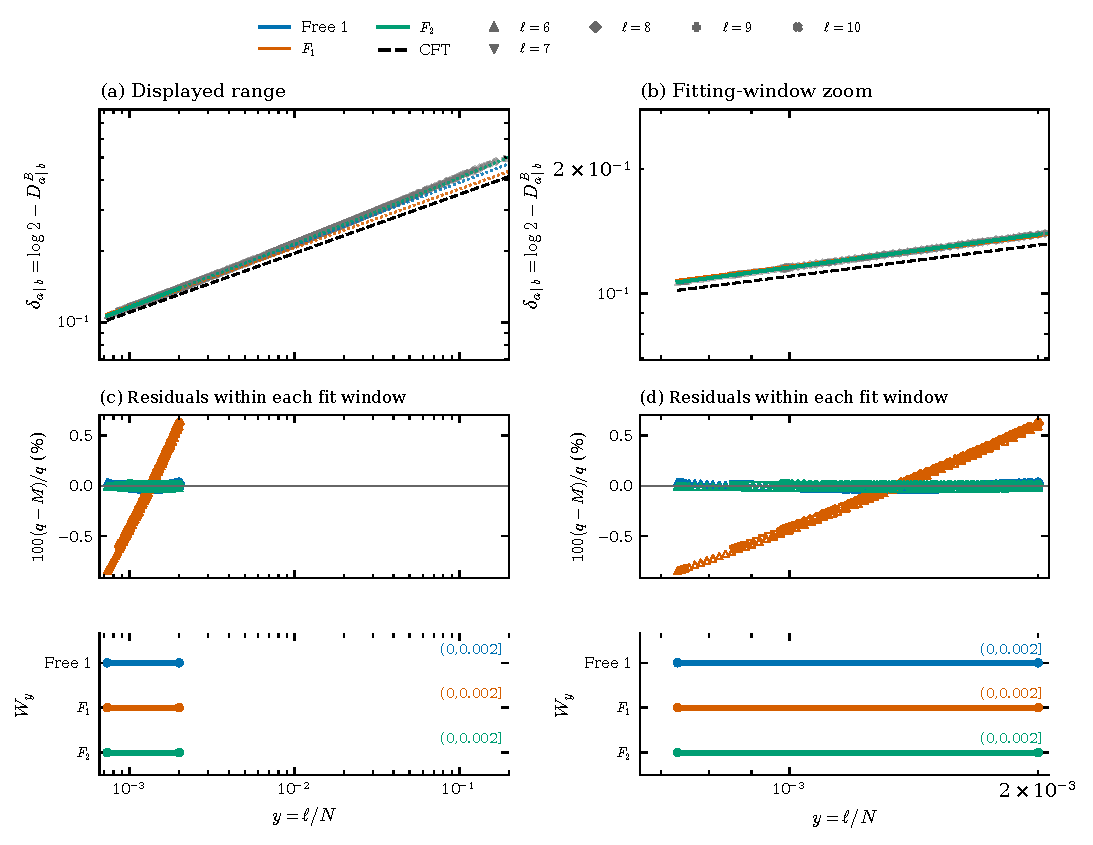
\includegraphics[width=.94\linewidth]{../figs/pair_large_ising_I_sigma.pdf}\par\smallskip
\begingroup\scriptsize\setlength{\tabcolsep}{4pt}
\begin{tabular}{lllrrrrr}\toprule
Set & Model & $W_z$ & $m$ & $c_0$ & $r^{(0)}$ & $c_1$ & $r^{(1)}$\\\midrule
Both & Free 1 & $(0,0.002]$ & 260 & 0.71994 & 0.2646516 & --- & ---\\
Both & $F_1$ & $(0,0.002]$ & 260 & 0.65339 & 0.25 & --- & ---\\
Both & $F_2$ & $(0,0.002]$ & 260 & 0.61463 & 0.25 & 0.20243 & 0.5\\
\midrule
Both & CFT & --- & --- & 0.61965 & 0.25 & --- & ---\\
\bottomrule\end{tabular}
\endgroup
\caption{Ising, large intervals, $I\mid \sigma$, at $p=1/2$, $\ell=6,\ldots,10$, and the complete size grid in Eq.~\eqref{eq:extended-grid}. Here $z=y$ and $q=\delta=\log2-D^B$. Left: all computed data through $z=0.20$; right: a zoom into the common fitting window. Both columns show the same Free 1, $F_1$, and $F_2$ fits. All six directions of this CFT and interval type use the same window. Gray markers denote the data. Colored solid segments lie inside each model\textquotesingle s fitting interval; dotted segments are extrapolations. Black dashed is the analytical CFT leading deficit. The observable axes are logarithmic and span the measured data; nonpositive predictions cannot appear there and out-of-range extrapolations leave the panel. Residual ordinates are linear and show $100(q-M)/q$ only on each model\textquotesingle s fitted observations. Bars give the exact fitting intervals. The parameter block follows Eq.~\eqref{eq:fit}, with $c_0,c_1$ multiplying $z^{r^{(0)}},z^{r^{(1)}}$; all coefficients include powers of $\pi$. A dash means an absent fitted term, or no fitting window for CFT. Values shown are rounded; curves use full precision.}
\label{fig:pair-large_ising-I-sigma}
\end{figure}
\begin{figure}[!htbp]\centering
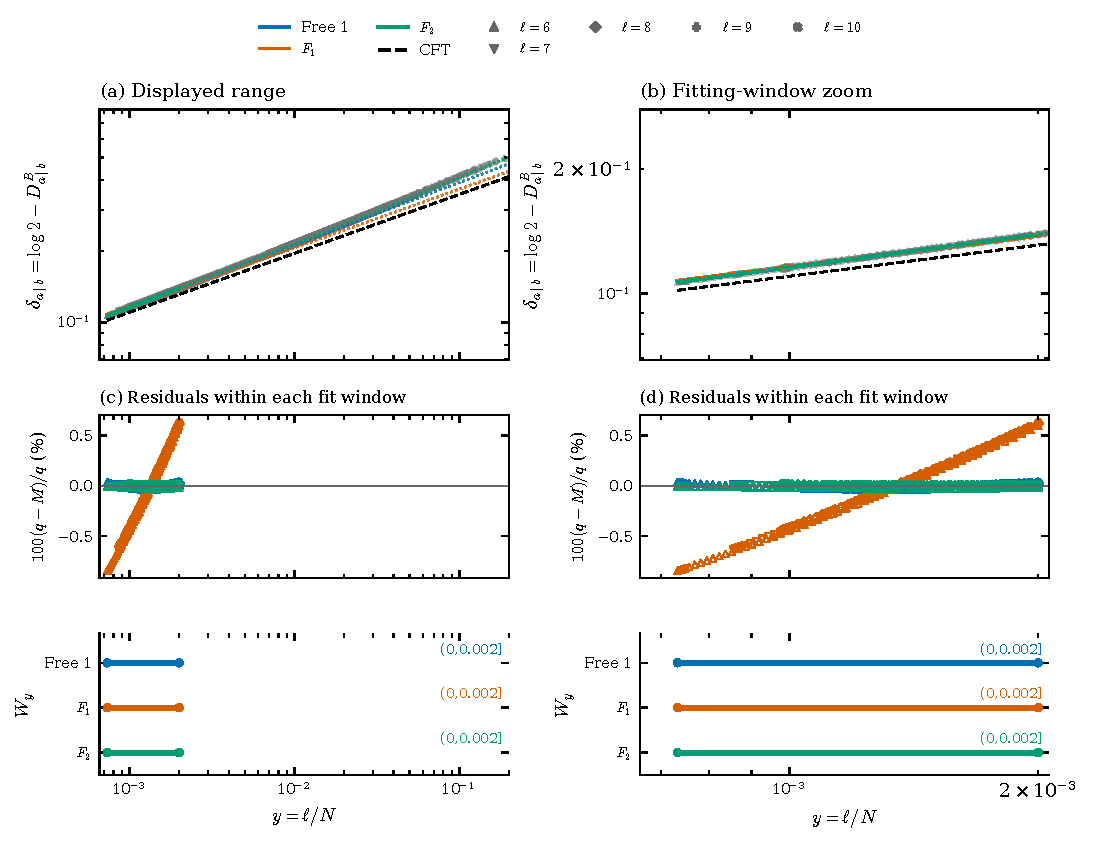
\includegraphics[width=.94\linewidth]{../figs/pair_large_ising_sigma_I.pdf}\par\smallskip
\begingroup\scriptsize\setlength{\tabcolsep}{4pt}
\begin{tabular}{lllrrrrr}\toprule
Set & Model & $W_z$ & $m$ & $c_0$ & $r^{(0)}$ & $c_1$ & $r^{(1)}$\\\midrule
Both & Free 1 & $(0,0.002]$ & 260 & 0.71995 & 0.2646531 & --- & ---\\
Both & $F_1$ & $(0,0.002]$ & 260 & 0.65339 & 0.25 & --- & ---\\
Both & $F_2$ & $(0,0.002]$ & 260 & 0.61462 & 0.25 & 0.20245 & 0.5\\
\midrule
Both & CFT & --- & --- & 0.61965 & 0.25 & --- & ---\\
\bottomrule\end{tabular}
\endgroup
\caption{Ising, large intervals, $\sigma\mid I$, at $p=1/2$, $\ell=6,\ldots,10$, and the complete size grid in Eq.~\eqref{eq:extended-grid}. Here $z=y$ and $q=\delta=\log2-D^B$. Left: all computed data through $z=0.20$; right: a zoom into the common fitting window. Both columns show the same Free 1, $F_1$, and $F_2$ fits. All six directions of this CFT and interval type use the same window. Gray markers denote the data. Colored solid segments lie inside each model\textquotesingle s fitting interval; dotted segments are extrapolations. Black dashed is the analytical CFT leading deficit. The observable axes are logarithmic and span the measured data; nonpositive predictions cannot appear there and out-of-range extrapolations leave the panel. Residual ordinates are linear and show $100(q-M)/q$ only on each model\textquotesingle s fitted observations. Bars give the exact fitting intervals. The parameter block follows Eq.~\eqref{eq:fit}, with $c_0,c_1$ multiplying $z^{r^{(0)}},z^{r^{(1)}}$; all coefficients include powers of $\pi$. A dash means an absent fitted term, or no fitting window for CFT. Values shown are rounded; curves use full precision.}
\label{fig:pair-large_ising-sigma-I}
\end{figure}
\begin{figure}[!htbp]\centering
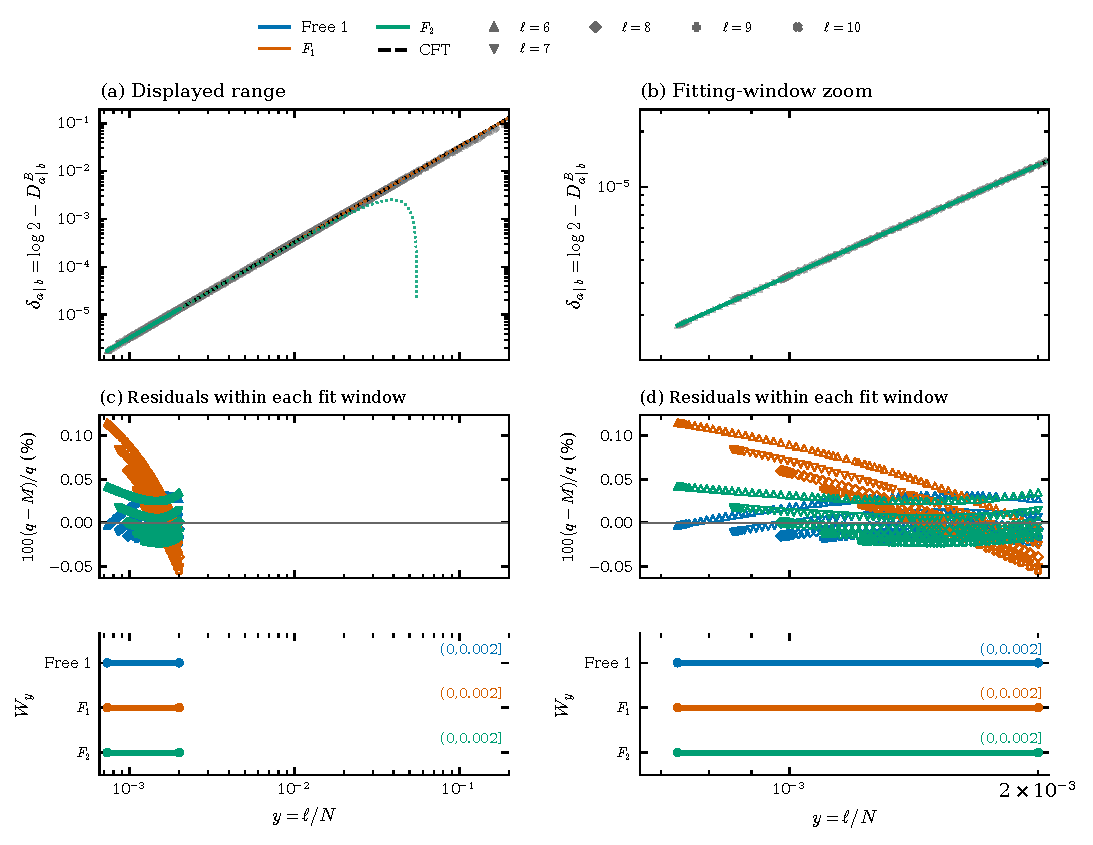
\includegraphics[width=.94\linewidth]{../figs/pair_large_ising_I_epsilon.pdf}\par\smallskip
\begingroup\scriptsize\setlength{\tabcolsep}{4pt}
\begin{tabular}{lllrrrrr}\toprule
Set & Model & $W_z$ & $m$ & $c_0$ & $r^{(0)}$ & $c_1$ & $r^{(1)}$\\\midrule
Both & Free 1 & $(0,0.002]$ & 260 & 3.2548 & 1.9985103 & --- & ---\\
Both & $F_1$ & $(0,0.002]$ & 260 & 3.2861 & 2 & --- & ---\\
Both & $F_2$ & $(0,0.002]$ & 260 & 3.289 & 2 & -1070.2 & 4\\
\midrule
Both & CFT & --- & --- & 3.2899 & 2 & --- & ---\\
\bottomrule\end{tabular}
\endgroup
\caption{Ising, large intervals, $I\mid \varepsilon$, at $p=1/2$, $\ell=6,\ldots,10$, and the complete size grid in Eq.~\eqref{eq:extended-grid}. Here $z=y$ and $q=\delta=\log2-D^B$. Left: all computed data through $z=0.20$; right: a zoom into the common fitting window. Both columns show the same Free 1, $F_1$, and $F_2$ fits. All six directions of this CFT and interval type use the same window. Gray markers denote the data. Colored solid segments lie inside each model\textquotesingle s fitting interval; dotted segments are extrapolations. Black dashed is the analytical CFT leading deficit. The observable axes are logarithmic and span the measured data; nonpositive predictions cannot appear there and out-of-range extrapolations leave the panel. Residual ordinates are linear and show $100(q-M)/q$ only on each model\textquotesingle s fitted observations. Bars give the exact fitting intervals. The parameter block follows Eq.~\eqref{eq:fit}, with $c_0,c_1$ multiplying $z^{r^{(0)}},z^{r^{(1)}}$; all coefficients include powers of $\pi$. A dash means an absent fitted term, or no fitting window for CFT. Values shown are rounded; curves use full precision.}
\label{fig:pair-large_ising-I-epsilon}
\end{figure}
\begin{figure}[!htbp]\centering
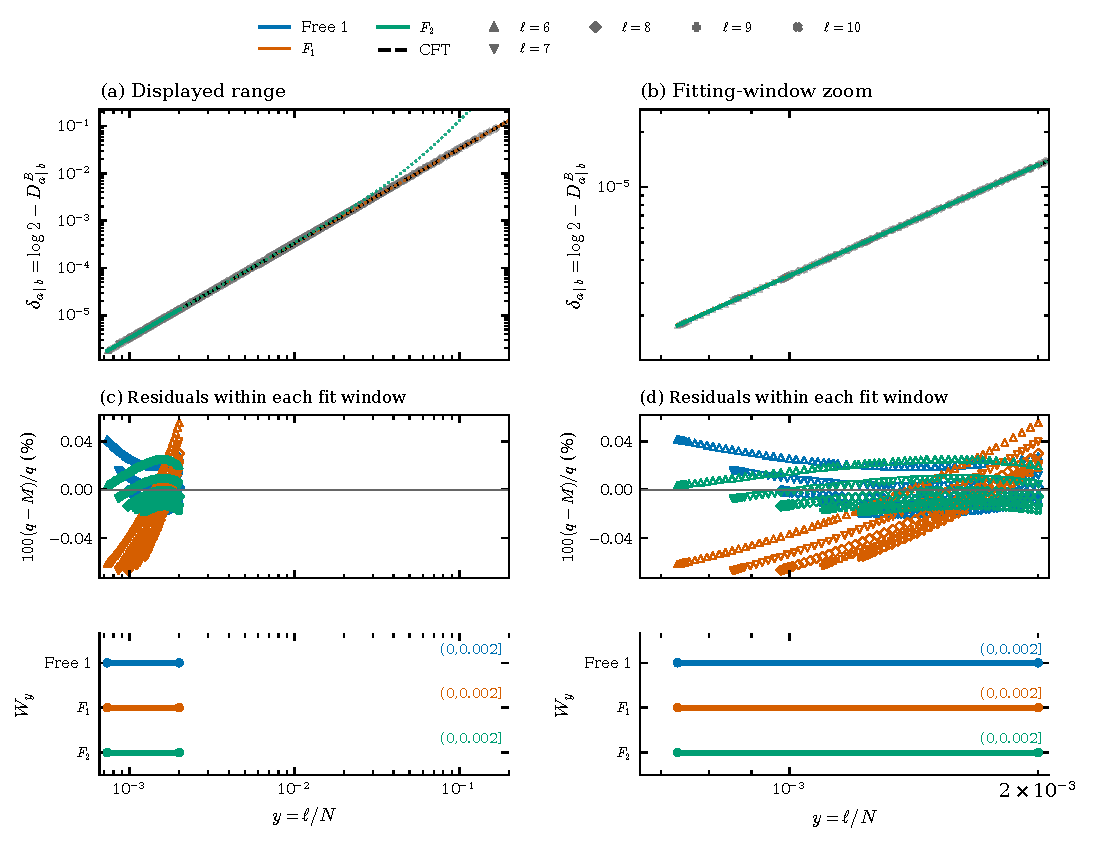
\includegraphics[width=.94\linewidth]{../figs/pair_large_ising_epsilon_I.pdf}\par\smallskip
\begingroup\scriptsize\setlength{\tabcolsep}{4pt}
\begin{tabular}{lllrrrrr}\toprule
Set & Model & $W_z$ & $m$ & $c_0$ & $r^{(0)}$ & $c_1$ & $r^{(1)}$\\\midrule
Both & Free 1 & $(0,0.002]$ & 260 & 3.3242 & 2.0013063 & --- & ---\\
Both & $F_1$ & $(0,0.002]$ & 260 & 3.2964 & 2 & --- & ---\\
Both & $F_2$ & $(0,0.002]$ & 260 & 3.2938 & 2 & 959.21 & 4\\
\midrule
Both & CFT & --- & --- & 3.2899 & 2 & --- & ---\\
\bottomrule\end{tabular}
\endgroup
\caption{Ising, large intervals, $\varepsilon\mid I$, at $p=1/2$, $\ell=6,\ldots,10$, and the complete size grid in Eq.~\eqref{eq:extended-grid}. Here $z=y$ and $q=\delta=\log2-D^B$. Left: all computed data through $z=0.20$; right: a zoom into the common fitting window. Both columns show the same Free 1, $F_1$, and $F_2$ fits. All six directions of this CFT and interval type use the same window. Gray markers denote the data. Colored solid segments lie inside each model\textquotesingle s fitting interval; dotted segments are extrapolations. Black dashed is the analytical CFT leading deficit. The observable axes are logarithmic and span the measured data; nonpositive predictions cannot appear there and out-of-range extrapolations leave the panel. Residual ordinates are linear and show $100(q-M)/q$ only on each model\textquotesingle s fitted observations. Bars give the exact fitting intervals. The parameter block follows Eq.~\eqref{eq:fit}, with $c_0,c_1$ multiplying $z^{r^{(0)}},z^{r^{(1)}}$; all coefficients include powers of $\pi$. A dash means an absent fitted term, or no fitting window for CFT. Values shown are rounded; curves use full precision.}
\label{fig:pair-large_ising-epsilon-I}
\end{figure}
\begin{figure}[!htbp]\centering
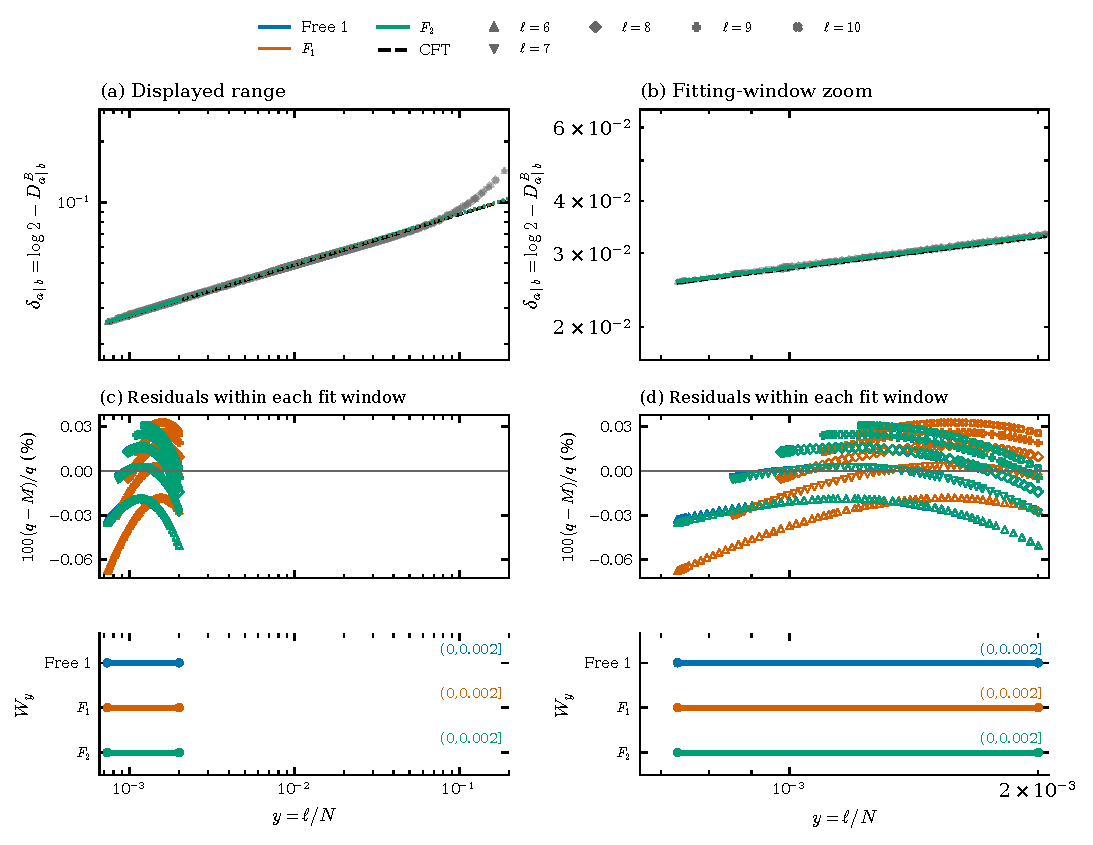
\includegraphics[width=.94\linewidth]{../figs/pair_large_ising_sigma_epsilon.pdf}\par\smallskip
\begingroup\scriptsize\setlength{\tabcolsep}{4pt}
\begin{tabular}{lllrrrrr}\toprule
Set & Model & $W_z$ & $m$ & $c_0$ & $r^{(0)}$ & $c_1$ & $r^{(1)}$\\\midrule
Both & Free 1 & $(0,0.002]$ & 260 & 0.15691 & 0.2505807 & --- & ---\\
Both & $F_1$ & $(0,0.002]$ & 260 & 0.15631 & 0.25 & --- & ---\\
Both & $F_2$ & $(0,0.002]$ & 260 & 0.15595 & 0.25 & 0.0018716 & 0.5\\
\midrule
Both & CFT & --- & --- & 0.15491 & 0.25 & --- & ---\\
\bottomrule\end{tabular}
\endgroup
\caption{Ising, large intervals, $\sigma\mid \varepsilon$, at $p=1/2$, $\ell=6,\ldots,10$, and the complete size grid in Eq.~\eqref{eq:extended-grid}. Here $z=y$ and $q=\delta=\log2-D^B$. Left: all computed data through $z=0.20$; right: a zoom into the common fitting window. Both columns show the same Free 1, $F_1$, and $F_2$ fits. All six directions of this CFT and interval type use the same window. Gray markers denote the data. Colored solid segments lie inside each model\textquotesingle s fitting interval; dotted segments are extrapolations. Black dashed is the analytical CFT leading deficit. The observable axes are logarithmic and span the measured data; nonpositive predictions cannot appear there and out-of-range extrapolations leave the panel. Residual ordinates are linear and show $100(q-M)/q$ only on each model\textquotesingle s fitted observations. Bars give the exact fitting intervals. The parameter block follows Eq.~\eqref{eq:fit}, with $c_0,c_1$ multiplying $z^{r^{(0)}},z^{r^{(1)}}$; all coefficients include powers of $\pi$. A dash means an absent fitted term, or no fitting window for CFT. Values shown are rounded; curves use full precision.}
\label{fig:pair-large_ising-sigma-epsilon}
\end{figure}
\begin{figure}[!htbp]\centering
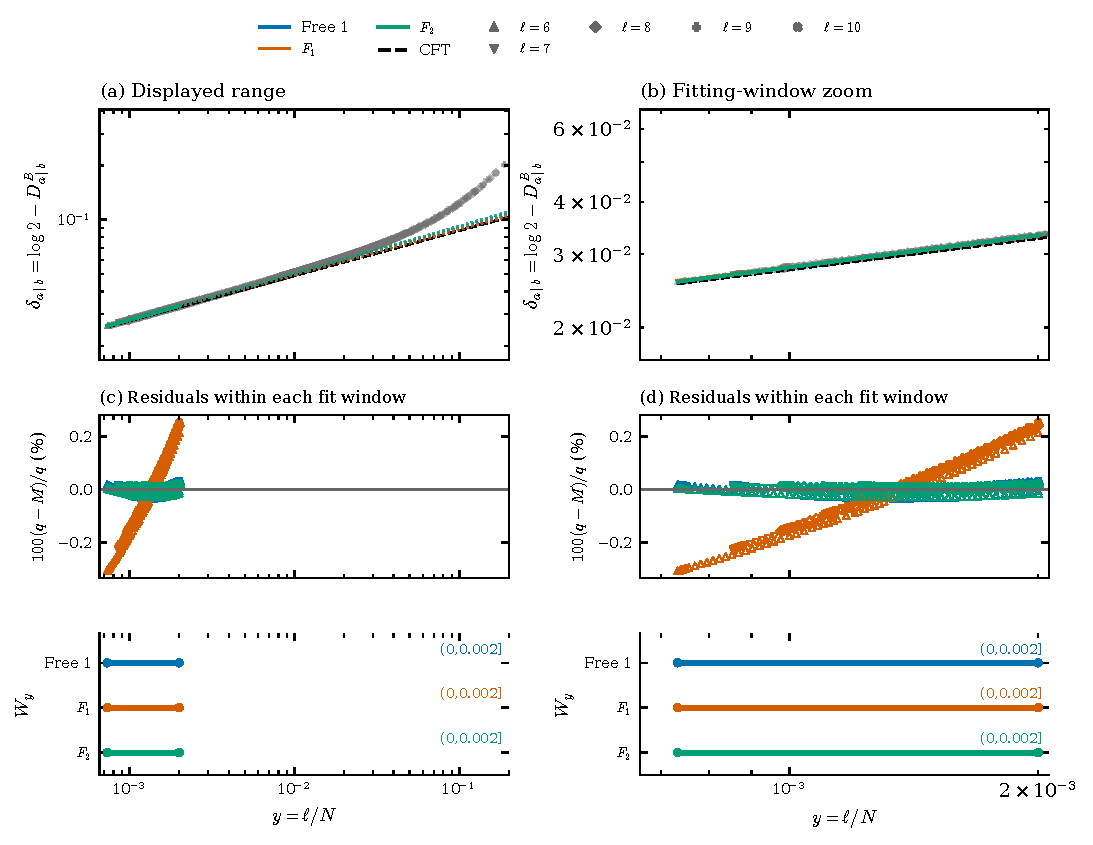
\includegraphics[width=.94\linewidth]{../figs/pair_large_ising_epsilon_sigma.pdf}\par\smallskip
\begingroup\scriptsize\setlength{\tabcolsep}{4pt}
\begin{tabular}{lllrrrrr}\toprule
Set & Model & $W_z$ & $m$ & $c_0$ & $r^{(0)}$ & $c_1$ & $r^{(1)}$\\\midrule
Both & Free 1 & $(0,0.002]$ & 260 & 0.16288 & 0.2554384 & --- & ---\\
Both & $F_1$ & $(0,0.002]$ & 260 & 0.15712 & 0.25 & --- & ---\\
Both & $F_2$ & $(0,0.002]$ & 260 & 0.15365 & 0.25 & 0.018087 & 0.5\\
\midrule
Both & CFT & --- & --- & 0.15491 & 0.25 & --- & ---\\
\bottomrule\end{tabular}
\endgroup
\caption{Ising, large intervals, $\varepsilon\mid \sigma$, at $p=1/2$, $\ell=6,\ldots,10$, and the complete size grid in Eq.~\eqref{eq:extended-grid}. Here $z=y$ and $q=\delta=\log2-D^B$. Left: all computed data through $z=0.20$; right: a zoom into the common fitting window. Both columns show the same Free 1, $F_1$, and $F_2$ fits. All six directions of this CFT and interval type use the same window. Gray markers denote the data. Colored solid segments lie inside each model\textquotesingle s fitting interval; dotted segments are extrapolations. Black dashed is the analytical CFT leading deficit. The observable axes are logarithmic and span the measured data; nonpositive predictions cannot appear there and out-of-range extrapolations leave the panel. Residual ordinates are linear and show $100(q-M)/q$ only on each model\textquotesingle s fitted observations. Bars give the exact fitting intervals. The parameter block follows Eq.~\eqref{eq:fit}, with $c_0,c_1$ multiplying $z^{r^{(0)}},z^{r^{(1)}}$; all coefficients include powers of $\pi$. A dash means an absent fitted term, or no fitting window for CFT. Values shown are rounded; curves use full precision.}
\label{fig:pair-large_ising-epsilon-sigma}
\end{figure}
